\documentclass[12pt,aspectratio=169,xcolor=dvipsnames]{beamer}
\usetheme{SimplePlus}
\usepackage{booktabs}
\usepackage{tikz}
\usepackage{pgfplots}
\usepackage{mathtools}

\newcommand{\R}{\mathbb{R}}
\newcommand{\N}{\mathbb{N}}

\title[short title]{Clase 12 Clases abstractas y operadores}
\subtitle{}
\author[NA Barnafi] {Nicolás Alejandro Barnafi Wittwer}
\institute[UC|CMM] 
{
    Pontificia Universidad Católica de Chile \\
    Centro de Modelamiento Matemático
}

\titlegraphic{
    \vspace{-1.8cm}
    \begin{flushright}
      
\includegraphics[height=2.5cm]{../images/puc.png} 
    \end{flushright}
}

\date{16/03/2024}
%\setbeamercovered{transparent}

\begin{document}
%%%%%%%%%%%%%%%%%%%%%%%%%%%%%%%%%%%%%%%%%%%%%%%%%%%%%%%
\begin{frame}
    \maketitle
\end{frame}
%%%%%%%%%%%%%%%%%%%%%%%%%%%%%%%%%%%%%%%%%%%%%%%%%%%%%%%
\begin{frame}{Clase de hoy}
    \begin{itemize}
        \item Motivación
        \item Espacios abstractos y su geometría
        \item Funciones, funciones de funciones, etc
    \end{itemize}

    \vspace{1cm}
    \newref{Spivak, Cálculo.}

    \newref{Algunos elementos del curso de análisis real.}
\end{frame}
%%%%%%%%%%%%%%%%%%%%%%%%%%%%%%%%%%%%%%%%%%%%%%%%%%%%%%%
\begin{frame}\frametitle{Contexto}
Quieren diseñar una plancha de cocina

    \begin{center}
        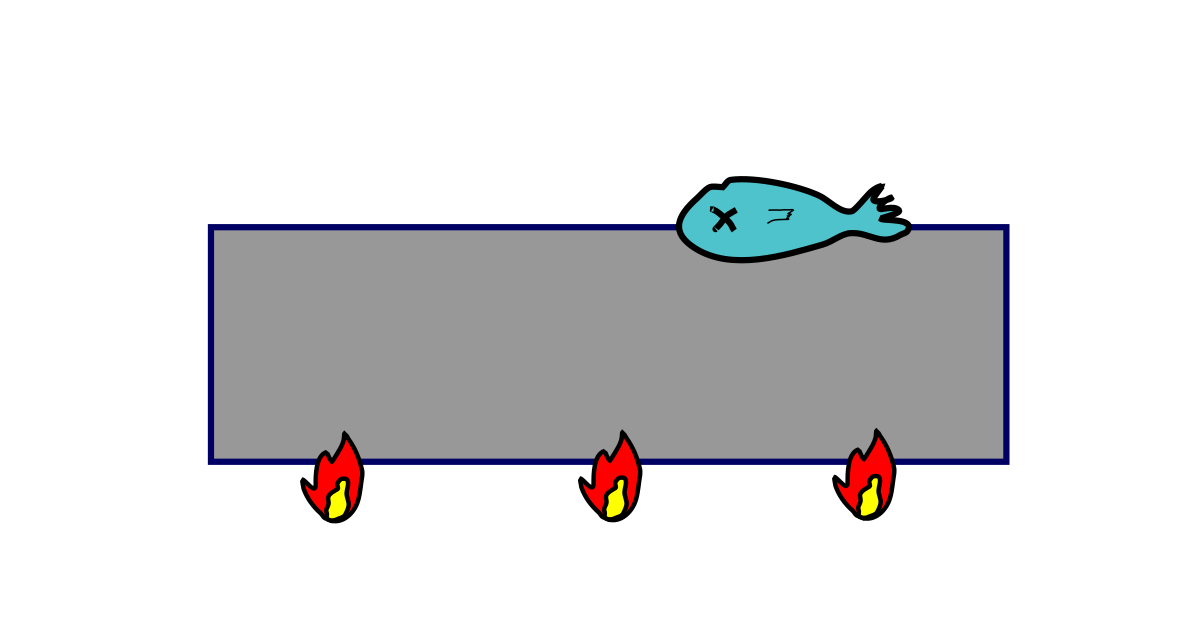
\includegraphics[width=0.5\textwidth]{../images/plancha.png}
    \end{center}
\end{frame}
%%%%%%%%%%%%%%%%%%%%%%%%%%%%%%%%%%%%%%%%%%%%%%%%%%%%%%%%%%%%%%%
\begin{frame}\frametitle{Problema I}
    Dada una temperatura de acción, qué temperatura alcanza?

    \begin{center}
        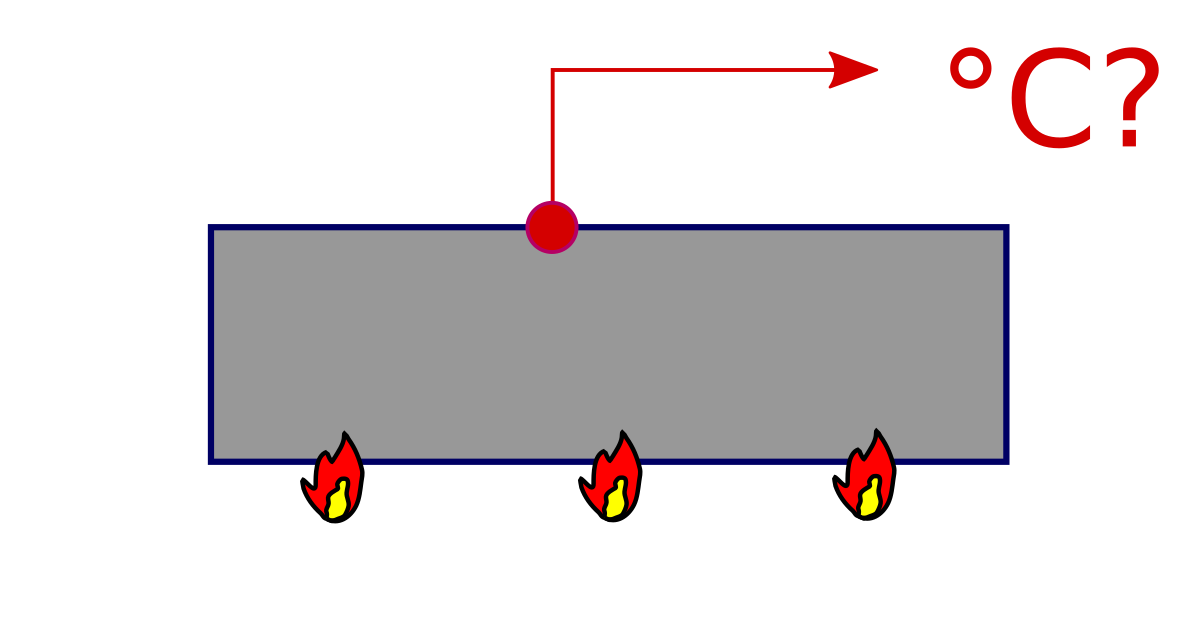
\includegraphics[width=0.5\textwidth]{../images/plancha-medida.png}
    \end{center}

\end{frame}
%%%%%%%%%%%%%%%%%%%%%%%%%%%%%%%%%%%%%%%%%%%%%%%%%%%%%%%%%%%%%%%
\begin{frame}\frametitle{Mediciones}
    \begin{center}
    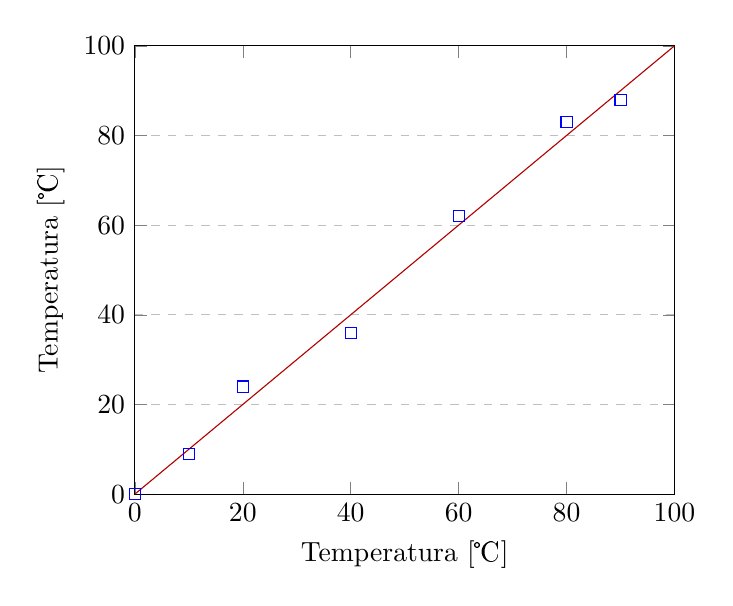
\begin{tikzpicture}
        \begin{axis}[
            title={}, xlabel={Temperatura [\textcelsius]}, ylabel={Temperatura [\textcelsius]},
            xmin=0, xmax=100,
            ymin=0, ymax=100,
            ymajorgrids=true,
            grid style=dashed,
            legend pos=south east
        ]

        \addplot[
            color=blue, only marks,
            mark=square,
            ]
            coordinates {
            (0,0)(10,9)(20,24)(40,36)(60,62)(80,83)(90,88)
            };

        \only<2>{\addplot [
            domain=0:100,
            samples=100,
            color=red!70!black,
            ]
            {x};}
        %\legend{Mediciones, Ajuste}

\end{axis}
\end{tikzpicture}
\end{center}
\end{frame}
%%%%%%%%%%%%%%%%%%%%%%%%%%%%%%%%%%%%%%%%%%%%%%%%%%%%%%%%%%%%%%%
\begin{frame}\frametitle{Problema II}
    Y si quiero la \emph{distribución} de temperatura?

    \begin{center}
        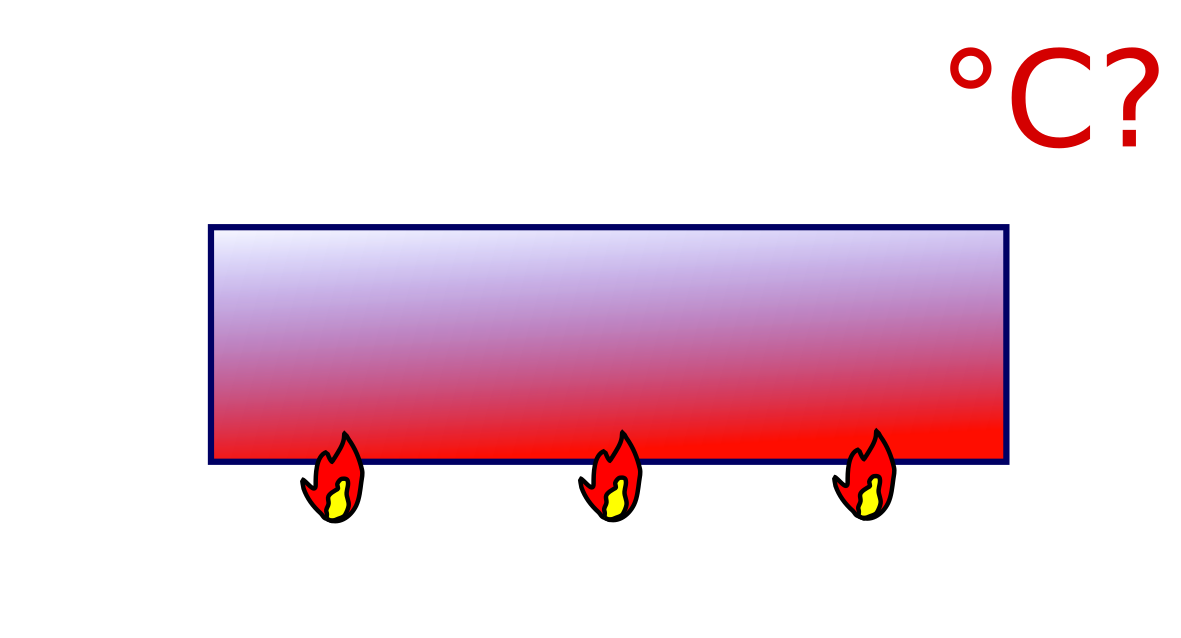
\includegraphics[width=0.5\textwidth]{../images/plancha-continuo.png}
    \end{center}

    \idea{Objeto de interés es una \emph{función} $T:\Omega\to \R$}
\end{frame}
%%%%%%%%%%%%%%%%%%%%%%%%%%%%%%%%%%%%%%%%%%%%%%%%%%%%%%%%%%%%%%%
%%%%%%%%%%%%%%%%%%%%%%%%%%%%%%%%%%%%%%%%%%%%%%%%%%%%%%%%%%%%%%%
\section{Espacios abstractos, funciones y funcionales}
%%%%%%%%%%%%%%%%%%%%%%%%%%%%%%%%%%%%%%%%%%%%%%%%%%%%%%%%%%%%%%%
%%%%%%%%%%%%%%%%%%%%%%%%%%%%%%%%%%%%%%%%%%%%%%%%%%%%%%%%%%%%%%%
\begin{frame}\frametitle{De funciones a funcionales}

    \begin{columns}[t]
        \begin{column}[t]{0.49\textwidth}
        {\bf Funciones}
        
            \begin{itemize}
                \item<+-> Van de un espacio a otro
                    $$ f: \mathbb R^3 \mapsto \mathbb R, f(x,y,z) = x+y-z $$
                \item<+-> Los puntos se pueden \emph{medir} (normados)
                    $$ |(x,y)| \coloneqq \sqrt{x^2+y^2} $$
                \item<+-> La norma permite medir distancias
                    $$ \text{dist}( \vec x_1, \vec x_2) \coloneqq |\vec x_1 - \vec x_2| $$
            \end{itemize}
        
        \end{column}

        \vline 
        \begin{column}[t]{0.49\textwidth}
        \,\,{\bf Funcionales}

            \begin{itemize}
                \item<+-> Van de un \emph{espacio funcional} a otro espacio
                \item<+-> Los espacios funcionales tienen \emph{normas} también 
                \item<+-> Con sus normas podemos medir distancias
            \end{itemize}
        \end{column}
    \end{columns}
\end{frame}
%%%%%%%%%%%%%%%%%%%%%%%%%%%%%%%%%%%%%%%%%%%%%%%%%%%%%%%%%%%%%%%
\begin{frame}[t]{Espacios vectoriales}
    Un espacio vectorial (real) $V$ es un espacio con una operación \emph{suma} $+:V\times V \to \R$ y una operación \emph{producto por escalar} $\cdot: \R\times V \to V$ tales que:
    \begin{itemize}
        \item Conmutatividad: $u+v=v+u$
        \item Asociatividad: $(u+v)+w =u+(v+w)$, $a\cdot(b\cdot v)=(a\cdot b)\cdot v$
        \item Neutro aditivo: $u + 0 = 0$
        \item Neutro multiplicativo: $1\cdot u = u$
        \item Inverso aditivo: Existe $-u\in V$ tal que $u + (-u) = 0$
        \item Distributividad: $(a+b)\cdot u = a\cdot u + b\cdot u$
    \end{itemize}
    
    \vspace{0.5cm}
    \idea{Ojo: no tiene el inverso multiplicativo}
\end{frame}
%%%%%%%%%%%%%%%%%%%%%%%%%%%%%%%%%%%%%%%%%%%%%%%%%%%%%%%%%%%%%%%
\begin{frame}{Ejercicio: definir suma y producto}
    \begin{itemize}
        \item Vectores $\R^d$
        \item Matrices $\R^{n\times m}$
        \item Sucesiones $a:\mathbb N\to \R$
        \item Sucesiones $a:\mathbb N \to \R$ convergentes ($\lim_{n\to\infty} a_n < \infty$)
        \item Funciones $f:\Omega_1 \subset \R^k \to \Omega_2\subset \R^l$
        \item Funciones continuas ($\lim_{x\to x_0} f(x) = f(x_0)$)
    \end{itemize}

    \vspace{1cm}
    \idea{En qué cambian los últimos dos pares?}
\end{frame}
%%%%%%%%%%%%%%%%%%%%%%%%%%%%%%%%%%%%%%%%%%%%%%%%%%%%%%%%%%%%%%%
\begin{frame}{Espacios funcionales}
    \begin{itemize}
        \item $\ell^p$ sucesiones $p$-sumables, i.e. $(a_n)_n$ tal que
                $$ \sum_i a_i^p < \infty $$
        \item $C(\R,\R)$: funciones continuas de $\R$ a $\R$
        \item $C^1(\R, \R)$: funciones diferenciables de $\R$ a $\R$
        \item $L^p(\R,\R)$ funciones $p$-integrables:
                $$\int_{-\infty}^\infty |f(x)|^p\,dx < \infty $$
    \end{itemize}
\end{frame}
%%%%%%%%%%%%%%%%%%%%%%%%%%%%%%%%%%%%%%%%%%%%%%%%%%%%%%%%%%%%%%%
\begin{frame}[t]\frametitle{Espacios funcionales}
    \begin{footnotesize}
    \begin{itemize}
        \item<+-> Podemos interpretar las funciones como puntos en estos espacios
            \begin{exampleblock}{}
                Sean $f_1, f_2$ dos funciones y $g = f_1 + f_2$. 

                Si $f_1(x) = x^2, f_2(x) = \sin(x), \quad\Rightarrow\quad g(x) = (f_1+f_2)(x) = f_1(x)+f_2(x) = x^2+\sin(x)$
            \end{exampleblock}
        \item<+-> Los espacios funcionales tienen \emph{normas} para cuantificar elementos\footnote{Contenido de Análisis Real}
            \begin{itemize}
                \item<+-> Espacio de funciones continuas de $\R$ a $\R$, $C(\R, \R)$. Si $f\in C(\R, \R)$, 
                    $$ \| f \|_{C(\R, \R)} \coloneqq \sup_{\vec x\in  \R^n}|f(x)|_{\R^m} $$
                \item<+-> Espacio de funciones cuadrado integrable\footnote{Por estudiar en Teoría de Integración} de $(0,1)$ a $\R$, $L^2((0,1), \R)$,
                    $$ \| f \|_{L^2((0,1), \R)} \coloneqq \left[ \int_0^1|f(x)|^2\,dx \right]^{1/2} $$
            \end{itemize}
    \end{itemize}
    \end{footnotesize}
\end{frame}
%%%%%%%%%%%%%%%%%%%%%%%%%%%%%%%%%%%%%%%%%%%%%%%%%%%%%%%%%%%%%%%
\begin{frame}{Ejemplos}
    \begin{itemize}
        \item<+-> $f(x) = 1/x$ con $f:\R \to \R$
            $$ \| 1/x \|_{C(\R, \R)} =\sup_{x\in \R} |1/x| = \infty$$
        \item<+-> $f(x) = 1/x$ con $f:[1,\infty) \to \R$
            $$\|1/x\|_{C([1,\infty),\R)} = \sup_{x\in [1,\infty)}|1/x| = 1 $$
    \end{itemize}

    \idea{Calcular $\| x^2 \|_{L^2((-1,1))}$, donde $\|\cdot\|_{L^2(\Omega)}=(\int_\Omega |\cdot|^2\,dx)^{1/2}$ }


\end{frame}
%%%%%%%%%%%%%%%%%%%%%%%%%%%%%%%%%%%%%%%%%%%%%%%%%%%%%%%%%%%%%%%
\begin{frame}\frametitle{Funcionales y operadores}
    Un \emph{funcional} toma una función y entrega un escalar. Un \emph{operador} toma una función y entrega una función\footnote{Contenido de Análisis Funcional}.  \pause

    \begin{itemize}
        \item<+-> Elevar función al cuadrado: $Q: C(\R, \R) \to C(\R, \R)$
            $$ Q[f] \coloneqq f^2, \quad Q[f](x) = f^2(x) $$
        \item<+-> La integral (definida): $I: L^2((0,1), \R) \to \R$
            $$ I[f] \coloneqq \int_0^1 f\,dx $$
        \item<+-> La derivada: $D: C^k(\R^n, \R) \to C^{k-1}(\R^n, \R^n)$
            $$ Df \coloneqq \nabla f, \quad [Df(x)]_i = \frac{\partial f}{\partial x_i}(x) $$
    \end{itemize}
\end{frame}
%%%%%%%%%%%%%%%%%%%%%%%%%%%%%%%%%%%%%%%%%%%%%%%%%%%%%%%
\begin{frame}{Pregunta abierta}
        $$ T:X\to Y $$
    Cómo se mide la continuidad de un operador...?
\end{frame}
%%%%%%%%%%%%%%%%%%%%%%%%%%%%%%%%%%%%%%%%%%%%%%%%%%%%%%%
\begin{frame}
    \maketitle
\end{frame}
%%%%%%%%%%%%%%%%%%%%%%%%%%%%%%%%%%%%%%%%%%%%%%%%%%%%%%%
\end{document}
